\chapter{Task 3 --- Ten-Epoch Training and Validation Analysis}
\label{ch:task3}

%-------------------------------------------------------

Task 3 asks for the training and validation loss and accuracy of the
baseline over the 10 epochs, the epoch-level macro-F1, and a discussion
of convergence, the training--validation gap and any over- or
underfitting. Only epoch-level summaries are used here.

At the end of every epoch, the training split (48,000 images) and the
validation split (12,000 images) were evaluated with the same weights in
evaluation mode (Section \ref{sec:loop}). Table \ref{table:epochs} lists
the values, and Figures \ref{fig:epochs-loss}--\ref{fig:epochs-f1} plot
them.

\begin{table}[h]
    \centering
    \caption[Baseline epoch-level metrics.]%
    {Baseline (SGD, $\eta = 0.01$, batch size 64): epoch-level loss,
    accuracy and macro-F1 on the training and validation splits.}

    \begin{tabular}{c|c|c|c|c|c|c}
        \specialrule{1.5pt}{0pt}{0pt}
        Epoch & Train loss & Train acc. & Train F1 & Val. loss & Val. acc. & Val. F1 \\
        \hline\hline
        1  & 0.0903 & 97.23\% & 0.9722 & 0.1084 & 96.75\% & 0.9673 \\
        2  & 0.0575 & 98.14\% & 0.9812 & 0.0724 & 97.78\% & 0.9776 \\
        3  & 0.0431 & 98.61\% & 0.9859 & 0.0693 & 97.83\% & 0.9781 \\
        4  & 0.0413 & 98.67\% & 0.9866 & 0.0643 & 98.27\% & 0.9826 \\
        5  & 0.0261 & 99.16\% & 0.9915 & 0.0557 & 98.31\% & 0.9829 \\
        6  & 0.0227 & 99.28\% & 0.9927 & 0.0574 & 98.29\% & 0.9827 \\
        7  & 0.0136 & 99.58\% & 0.9958 & \textbf{0.0425} & \textbf{98.77\%} & \textbf{0.9876} \\
        8  & 0.0131 & 99.59\% & 0.9959 & 0.0473 & 98.63\% & 0.9862 \\
        9  & 0.0248 & 99.11\% & 0.9909 & 0.0558 & 98.54\% & 0.9853 \\
        10 & 0.0129 & 99.56\% & 0.9956 & 0.0473 & 98.68\% & 0.9867 \\
        \specialrule{1.5pt}{0pt}{0pt}
    \end{tabular}
    \label{table:epochs}
\end{table}

\begin{figure}[H]
    \centering
    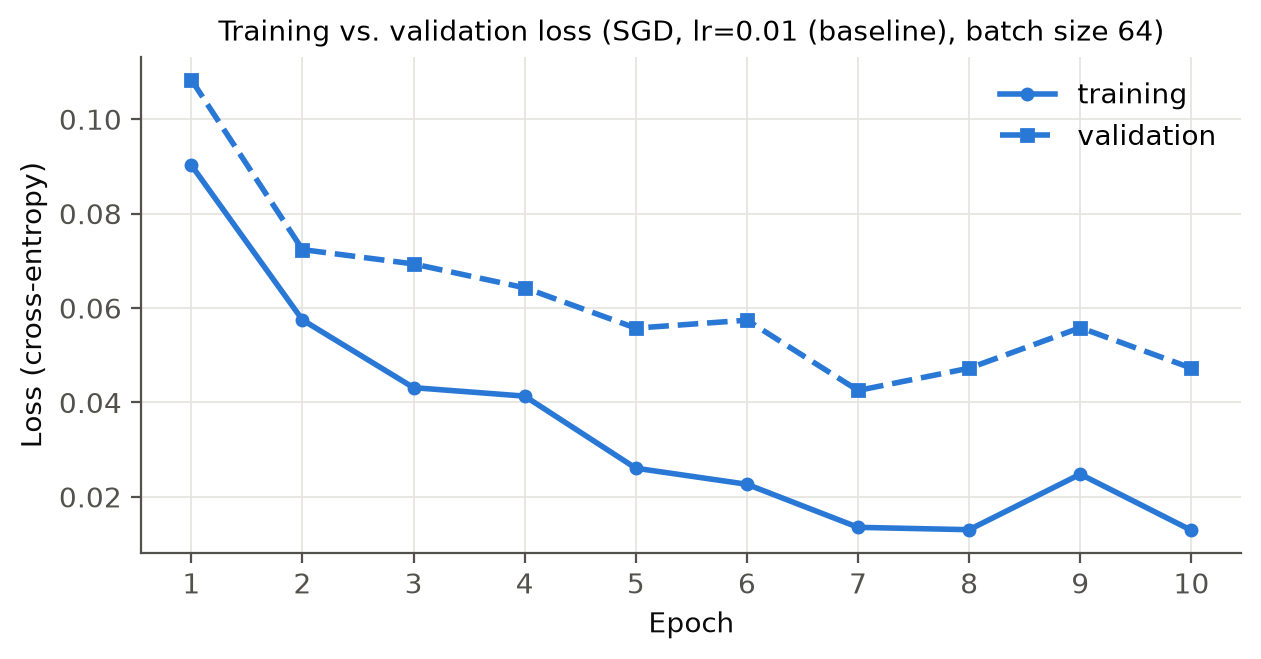
\includegraphics[width = 0.88\textwidth]{epochs_loss.png}
    \caption[Training and validation loss over 10 epochs.]%
    {Baseline: training and validation cross-entropy loss per epoch.}
    \label{fig:epochs-loss}
\end{figure}

\begin{figure}[H]
    \centering
    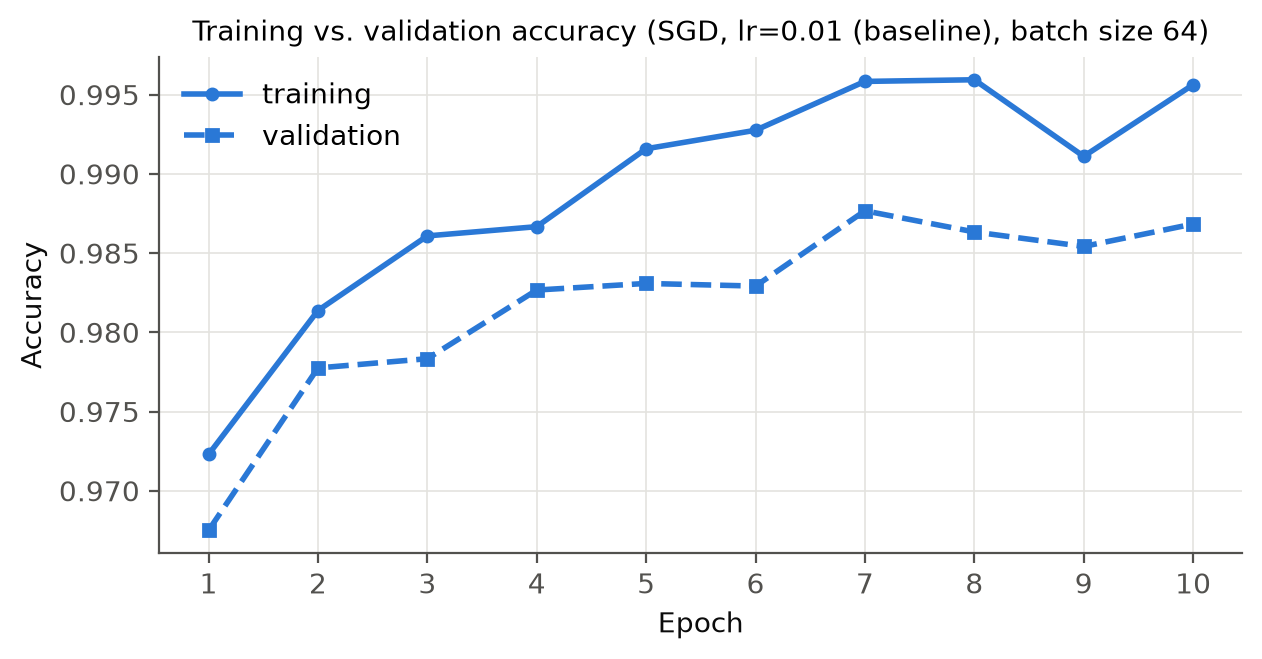
\includegraphics[width = 0.88\textwidth]{epochs_accuracy.png}
    \caption[Training and validation accuracy over 10 epochs.]%
    {Baseline: training and validation accuracy per epoch.}
    \label{fig:epochs-acc}
\end{figure}

\begin{figure}[H]
    \centering
    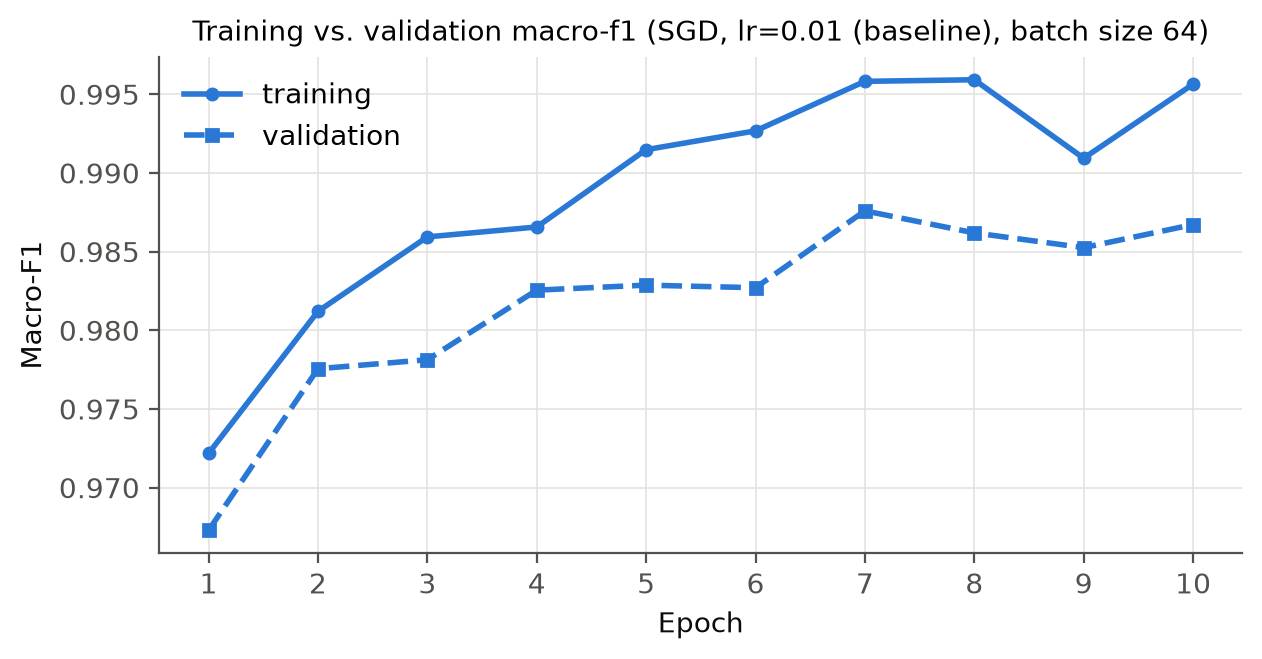
\includegraphics[width = 0.88\textwidth]{epochs_f1.png}
    \caption[Training and validation macro-F1 over 10 epochs.]%
    {Baseline: training and validation macro-F1 per epoch.}
    \label{fig:epochs-f1}
\end{figure}

\textbf{Convergence.} Most of the learning happens in the first epoch:
after it, validation accuracy is already 96.75\%. The next epochs add
smaller gains, and validation accuracy stays between 98.27\% and
98.77\% from epoch 4 on. The best validation epoch is epoch 7 (loss
0.0425, accuracy 98.77\%). After that the validation curves stop
improving and move up and down within about 0.25 percentage points, so
the model has converged by about epoch 7. Epoch 9 shows a small
bump: training loss rises from 0.0131 to 0.0248 and validation loss from
0.0473 to 0.0558, and both recover in epoch 10. With a constant
learning rate and momentum, a few unlucky batches can push the weights
slightly away from a good point. The training and validation curves
move together here, so I read it as optimization noise. Overfitting
would show up as validation loss rising while training loss falls.

\textbf{Training--validation gap.} Training is better than validation at
every epoch, and the gap grows over time. In accuracy it goes from 0.48
percentage points at epoch 1 to 0.88 points at epoch 10; in loss, the
training loss at epoch 10 (0.0129) is less than a third of the
validation loss (0.0473). Macro-F1 follows accuracy almost exactly on
both sets (differences of at most 0.0002), so the errors are spread
across the digits.

\textbf{Overfitting and underfitting.} There is no underfitting: the
network reaches 99.6\% training accuracy, so it has enough capacity for
this task. There is \emph{mild} overfitting after epoch 7: the training
loss keeps going down while the validation loss stops improving (0.0425
at epoch 7, then 0.047--0.056), so the extra epochs mostly fit the
training images more tightly. The effect is small, though. Validation
accuracy does not drop in any meaningful way (98.68\% at epoch 10
against 98.77\% at its best), and the final model still generalizes
well. Dropout or weight decay could reduce the gap further, and early
stopping around epoch 7 would be another option.
